

\section{Vorstellung des Ergebnisses}

\subsection{Überblick}
%TO-DO: Eventuell noch mit ein paar Bildern anreichern
In diesem Kapitel soll das von uns entwickelte Spiel \enquote{RPG-Adventure} vorgestellt werden. Dazu wird zunächst ein Überblick über Konzept und Spielablauf anhand des unten zu sehenden Ablaufdiagramms \ref{fig:2022-01-08-Spielablauf-Chart} gegeben. Darauf folgen nähere Erläuterungen zu verschiedenen Teilaspekten des Spiels, wie Gamedesign, Grafikdesign, Frontend und Backend. 

In \enquote{RPG-Adventure} übernimmt der Spieler die Rolle eines Söldners, der durch das Land zieht und sein Geld als Monsterjäger verdient (ähnlich dem \enquote{Witcher} aus den Romanen von Andrzej Sapkowski). Das Spiel besitzt sowohl Einzelspieler- als auch Mehrspielerkomponenten. Letztere sind auf eine Art und Weise konzipiert, die ein erfolgreiches Bestreiten der Inhalte nur durch Zusammenarbeit mit anderen Spielern möglich macht. Kommunikation und Kooperation mit den Mitspielern sind hier erwünscht und notwendig. 

Nach der Anmeldung auf der Website erhält der Spieler die Möglichkeit sich einen (oder mehrere) Charakter(e) zu erstellen. Diesen Charaktere kann eine von drei verfügbaren Klassen zugewiesen werden: Krieger, Priester und Zauberer. Diese Klassen besitzen die Attribute Lebenspunkte (HP) und Angriffskraft (AP), welchen je nach Klasse feste Startwerte zugewiesen sind. Mithilfe von Erfahrungspunkten (XP) können diese Attribute während im Spielverlauf gesteigert werden. Außerdem hat jede Klasse eine Spezialfähigkeit, die im Kampf eingesetzt werden kann. Das taktische Einsetzen dieser Fähigkeiten kann im Spiel für Sieg oder Niederlage entscheidend sein.

Die Klassen unterscheiden sich wie folgt:

\begin{itemize}
    \item Krieger
    \begin{itemize}
        \item Rolle:        Tank 
        \item Startwerte:   200 HP, 15 AP 
        \item Fähigkeit:    Verringert Angriffspunkte des Gegners
    \end{itemize}
    \item Priester
    \begin{itemize}
        \item Rolle:        Heiler
        \item Startwerte:   75 HP, 5 AP
        \item Fähigkeit:    Heilt sich selbst und die Gruppe
    \end{itemize}
    \item Zauberer
    \begin{itemize}
        \item Rolle:        Schaden
        \item Startwerte:   100 HP, 25 Aspekte
        \item Fähigkeit:    Erhöht die Angriffspunkte der Gruppe
    \end{itemize}
\end{itemize}

Nach Abschluss der Charaktererstellung kann der Spieler die Weltkarte betreten. Auf der Karte sind eine Reihe von Orten hervorgehoben, die verschiedene Level (im Kontext der Entwicklung Szenen genannt) darstellen und von dem Spieler betreten werden können. Innerhalb dieser Level ist es die Aufgabe des Spielers/der Spieler einen Gegner im Kampf zu bezwingen. Es gibt drei Einzelspieler- und zwei Mehrspieler-Level. Die drei Einzelspieler-Level werden nacheinander freigeschaltet und besitzen einen aufsteigenden Schwierigkeitsgrad. Schließt der Spieler alle drei erfolgreich ab, ist das Spiel zum jetzigen Entwicklungsstand durchgespielt. Die Mehrspieler-Level sind deutlich schwieriger, aber optional. Hier hat der Spieler auf der Weltkarte die Möglichkeit mithilfe eines globalen Chats Mitstreiter zu finden. Alle Level sind zudem beliebig oft wiederholbar.

Es gibt folgende Level:
\begin{itemize}
    \item Einzelspieler
    \begin{itemize}
        \item Level 1:  Am Rande des Dunkelwaldes; Gegner: Warg
        \item Level 2:  Das Alte Anwesen; Gegner: Vampirfürst
        \item Level 3:  Der Ascheberg; Gegner: Drache
    \end{itemize}
    \item Mehrspieler
    \begin{itemize}
        \item Level 4:  Der Friedhof in den Sümpfen, Gegner: Untoter
        \item Level 5:  Die verlassene Mine; Gegner: Wurm
    \end{itemize}
\end{itemize}

Wenn der Spieler sich für ein Level entschieden hat, wird er in eine Lobby weitergeleitet. Auch hier kann über ein Chatfenster mit anderen Spielern in der Lobby kommuniziert werden. Jedes Level hat eine feste Anzahl von Spielerslots, die mit Klick auf einen entsprechenden Button \enquote{belegt} werden können. Sind alle Spielerslots belegt, startet ein Countdown und der Spieler das Level betreten. 

Im Level angekommen steht dem Spieler ein Bossgegner gegenüber den es zu besiegen gilt. Der Kampfbildschirm ist aufgeteilt in eine Grafik des Gegners mit einem animierten Sprite und Hintergrund, einen Status- und Aktionsbereich für den Spieler, ein Gamelog und ein Inputfeld für Chatnachrichten (welche im Gamelog angezeigt werden). Kämpfe laufen rundenbasiert ab, wobei der Gegner immer zuerst an der Reihe ist. Hat dieser seine Aktion ausgeführt, wartet das Spiel auf die Aktion des Spielers. Dieser hat nun die Möglichkeit entweder einen Angriff auszuführen oder seine Klassenfähigkeit einzusetzen. Ein Aussetzen ist ebenfalls möglich.
Handelt es sich um einen Mehrspieler-Kampf, wartet das Spiel auf die Eingabe aller beteiligten Spieler, bevor die Runde voranschreitet. Im Gamelog wird kenntlich gemacht, wenn Spieler ihre Aktionen ausgewählt haben und auf die Eingabe der anderen warten. 
Die Stärke des Angriffs von Spielern und Gegner ergibt sich aus den Angriffspunkten des jeweiligen Charakters und einer darauf basierenden Zufallskomponente.

Der Kampf endet, wenn die Lebenspunkte des Bossgegners oder die aller beteiligten Spieler auf 0 fallen. Der erste Fall resultiert in einem Sieg für die Spieler, die nun Erfahrungspunkte erhalten. Der zweite Fall resultiert in einer Niederlage mit einem stark verminderten Erhalt von Erfahrungspunkten. In beiden Fällen werden die Spieler zu einem Spielabschluss-Bildschirm weitergeleitet von wo aus die Rückkehr zur Weltkarte oder in die Charakterauswahl möglich ist. Die erhaltenen Erfahrungspunkte können jetzt genutzt werden, um die Charakterattribute zu verbessern und auf der Weltkarte können weitere Level ausgewählt werden.
%TO-DO: Diagramm muss geupdatet werden

\begin{figure}[H]
    \centering
    \caption{Diagramm: Seitenaufbau und Spielablauf}
    \label{fig:2022-01-08-Spielablauf-Chart}
    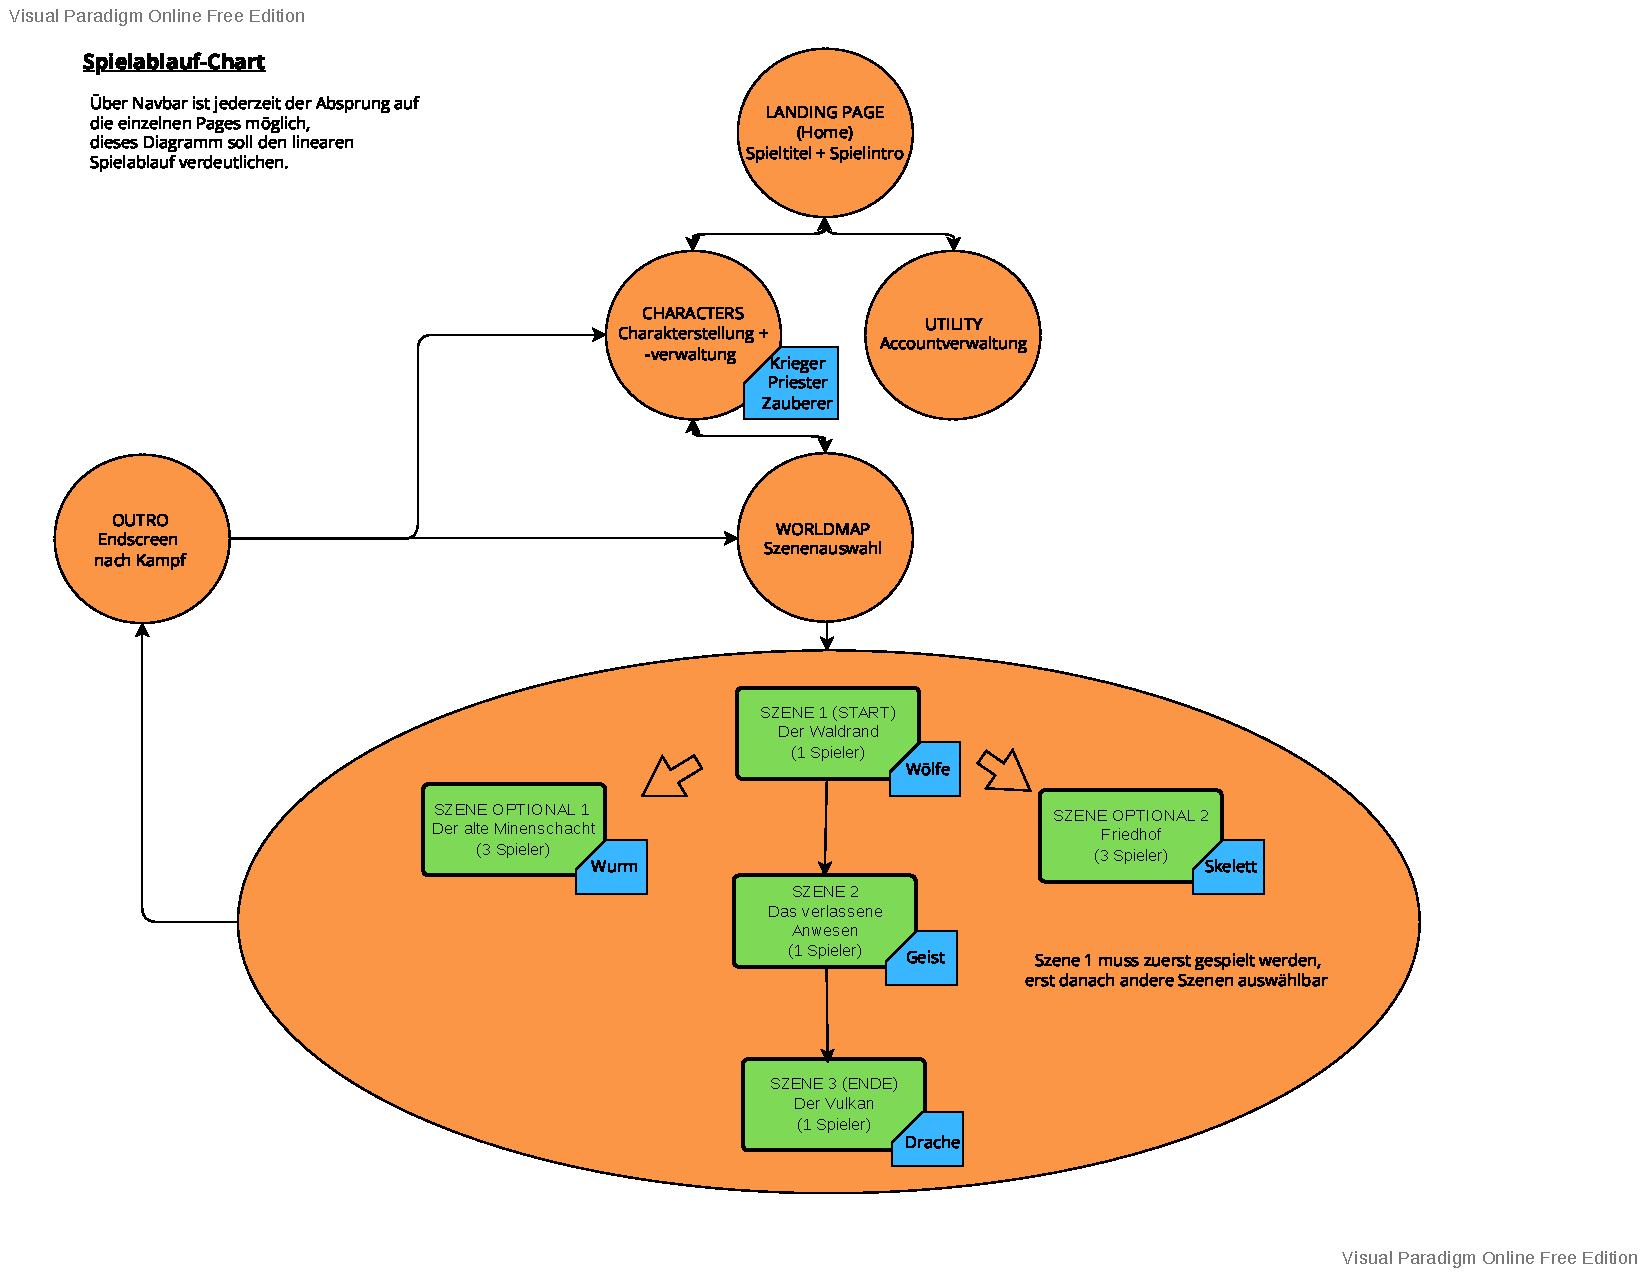
\includegraphics[width=1\textwidth, height=10cm]{2022-01-08-Spielablauf-Chart}
\end{figure}

Abschließend sei erwähnt, dass sich das Spiel in gewisser Weise in einem \enquote{Alpha}-Status befindet. Alle oben beschriebenen Inhalte wurden planmäßig umgesetzt und funktionieren grundsätzlich auch. Der \enquote{Veröffentlichung} des Spiels ist allerdings keine eingehende Testphase vorausgegangen, etwaige Spielfehler können also nicht gänzlich ausgeschlossen werden. Refactoring wurde auch nur sehr rudimentär betrieben, da der Programmcode bis kurz vor \enquote{Veröffentlichung} noch häufigen Änderungen unterworfen war.

